\documentclass{beamer}

\usepackage{tikz}
\usepackage{graphicx}

\begin{document}

\title{Frequent-Collision Blockchains for Local Geographic Authentication}
\author{Ryan Robinett and Tiago Royer}
\date{12 Nov 2019}
\institute[CMSC33300]{
    CMSC33300 --- Networks \\
    Department of Computer Science \\
    University of Chicago
}

\begin{frame}
    \titlepage
\end{frame}

\begin{frame}
	\frametitle{Problem motivation}

	\begin{itemize}
		\item Geographic Authentication:
			proving you are/were in a certain location
			at a certain point in time
		\item Problems with centralization
			\begin{itemize}
				\item Single point of failure
				\item Falsification of data
				\item Preservation of data
			\end{itemize}
		\item Goal: decentralized, historic geographic authentication
			\begin{itemize}
				\item Conventional geographic authentication asks, \textbf{``Where are you now?''}
				\item We want to ask, \textbf{``Where have you been in the recent past?''}
			\end{itemize}
	\end{itemize}
\end{frame}

\begin{frame}
	\frametitle{Blockchain as decentralized ledger (Decker 2013)}
	\begin{columns}
		\begin{column}{0.3\textwidth}
			\begin{figure}
				\centering
				\includegraphics[width=\textwidth]{decker_figures/decker_3.png}
				\includegraphics[width=\textwidth]{decker_figures/decker_5.png}
				\includegraphics[width=\textwidth]{decker_figures/decker_7.png}
			\end{figure}
		\end{column}

		\begin{column}{0.7\textwidth}
			\begin{itemize}
				\item In Bitcoin network, the time between creation of subsequent blocks follows an exponential distribution
				\begin{itemize}
					\item $p(t_{i+1}-t_i)=\lambda e^{-\lambda\left(t_{i+1}-t_i\right)}$
				\end{itemize}
				\item The rate of block creation is controlled s.t. \textbf{forks} occur only in local chains
				\begin{itemize}
					\item These forks are resolved in small timescales with high probability
				\end{itemize}
				\item Propagating false blocks so as to adversarially control the global chain is (asymptotically) preventative as the chain grows
				\begin{itemize}
					\item Why an adversary has to control approx. 50\% of nodes to invalidate the ledger in case of Bitcoin
				\end{itemize}
			\end{itemize}
		\end{column}
	\end{columns}
\end{frame}

\begin{frame}
	\frametitle{Blockchains... with a twist!}
	\begin{columns}
		\begin{column}{0.3\textwidth}
			\hfil
			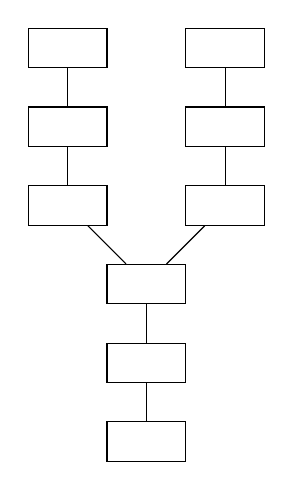
\begin{tikzpicture}[
					every node/.style = {
						shape = rectangle,
						draw,
						minimum width = 1cm,
						minimum height = 0.5cm,
					},
			]
				\draw (0, 0) node (a1) {};
				\draw (0, 1) node (a2) [rectangle] {};
				\draw (0, 2) node (a3) [rectangle] {};
				\draw (1, 3) node (b4) [rectangle] {};
				\draw (1, 4) node (b5) [rectangle] {};
				\draw (1, 5) node (b6) [rectangle] {};
				\draw (-1, 3) node (c4) [rectangle] {};
				\draw (-1, 4) node (c5) [rectangle] {};
				\draw (-1, 5) node (c6) [rectangle] {};

				\draw (a1) -- (a2);
				\draw (a2) -- (a3);
				\draw (a3) -- (b4);
				\draw (b4) -- (b5);
				\draw (b5) -- (b6);
				\draw (a3) -- (c4);
				\draw (c4) -- (c5);
				\draw (c5) -- (c6);
			\end{tikzpicture}
		\end{column}

		\begin{column}{0.7\textwidth}
			\begin{itemize}
				\item Each smartphone is a node
				\item \textbf{IDEA:} Create blocks at an exacerbatory rate
				\begin{itemize}
					\item \textbf{Local forks} still mitigated in short timescales
					\item \textbf{Global forks} forced to occur with high probability
					\item Each chain represents one geographical location
				\end{itemize}
				\item \textbf{EXPECTATION:} each \textbf{orphan chain} corresponds to a specific geographic clique
				\begin{itemize}
					\item While there is no global consensus, the rate of block creation enforces (locally) a decentralized ledger which requires approx. 50\% of local nodes to control
				\end{itemize}
			\end{itemize}
		\end{column}
	\end{columns}
\end{frame}

\begin{frame}
	\frametitle{Milestones}
	\begin{figure}
		\textbf{Milestones:} \\
		\vspace{3mm}
		\begin{tabular}{|r|l|}
			\hline
			Protocol design & in progress \\
			\hline
			Simulation of the blockchain & Done \\
			\hline
			Simulation of neighborhood dynamics & Done \\
			\hline
			Simulation of the protocol & November 23rd \\ % tentative
			\hline
			Analysis of first-order adversarial attacks & November 30th \\
			\hline
			Final presentation & December 10th \\
			\hline
		\end{tabular}
	\end{figure}
\end{frame}

\begin{frame}
	\frametitle{Supplementary Material: Transaction Primitives}
	\begin{figure}
		\scriptsize
		\centering
		\textbf{Transaction Primitives:} \\
		\vspace{5mm}
		\begin{description}
			\item[\textbf{Challenge Proposal:}] A challenge proposal $\mathcal{P}$ by
				node $C$ is a tuple of the form
				$$\mathcal{P}=(t_{\mathcal{P},C},\mathcal{C};\mathcal{P}^\prime_h,\mathcal{P}^\prime_t).$$
				Here:
				\begin{itemize}
					\item $t_{\mathcal{P},C}$ is the timestamp of $C$'s local clock upon
					creation of problem $\mathcal{P}$;
					\item $\mathcal{C}$ is the public key of node $C$;
					\item $\mathcal{P}^\prime_h$ is the header of block instance
					$\mathcal{P}^\prime$ (see below); and
					\item $\mathcal{P}^\prime_t$ is the tail of block instance
					$\mathcal{P}^\prime$. We refer to $\mathcal{P}^\prime$ as
					the \textbf{parent} of $\mathcal{P}$.
				\end{itemize}
				The tuple
				$\mathcal{P}=(t_{\mathcal{P},C},\mathcal{C};\mathcal{P}^\prime_h,\mathcal{P}^\prime_t)$
				naturally decomposes into the tuples
				$\mathcal{P}_h=(t_{\mathcal{P},C},\mathcal{C})$ and
				$\mathcal{P}_r=(\mathcal{P}^\prime_h,\mathcal{P}^\prime_t)$, which we
				refer to as the \textbf{header} and \textbf{reference tag} of $\mathcal{P}$,
				respectively.
			\item[\textbf{Block:}] A block $\mathcal{P}^*$ is a challenge proposal instance
				$\mathcal{P}=(t_{\mathcal{P},C},\mathcal{C};\mathcal{P}^\prime_h,\mathcal{P}^\prime_t)$
				together with the tuple $\mathcal{P}_t=(t_{\mathcal{P},S},\mathcal{S},n_{\mathcal{P},S})$.
				We refer to $\mathcal{P}^*_t$ as the \textbf{footer} of $\mathcal{P}^*$.
		\end{description}
	\end{figure}
\end{frame}

\end{document}
